\documentclass{standalone}
\usepackage{pgf}
\usepackage{tikz}
\usepackage{amsmath,amssymb}
\newcommand{\mt}[1]{\ensuremath{\mathbf{#1}}}
\newcommand{\vc}[1]{\ensuremath{\boldsymbol{#1}}}



\usetikzlibrary{arrows,automata,matrix}
\usepackage[latin1]{inputenc}
\begin{document}

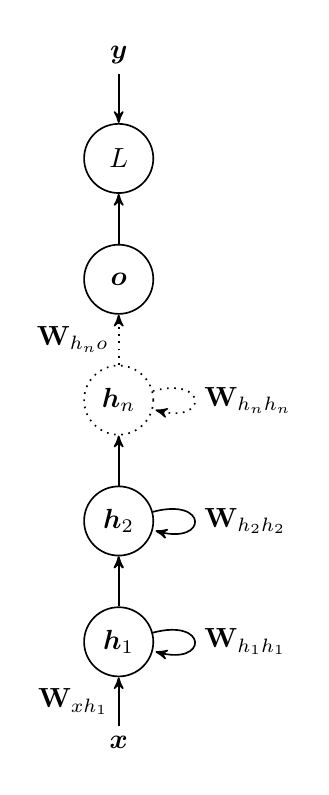
\begin{tikzpicture}[->,>=stealth'
  ,shorten >=0pt
  ,auto,node distance=4cm,
  semithick]
  \tikzstyle{every state}=[]

  \matrix (m) [matrix of nodes
  ,row sep=.25in,column sep=.25in] {
    \node[     ](y) {$\vc{y}$}; \\
    \node[state](L) {$L$}; \\
    \node[state](o) {$\vc{o}$}; \\
    \node[state,dotted](hn) {$\vc{h}_n$}; \\
    \node[state](h2) {$\vc{h}_2$}; \\
    \node[state](h1) {$\vc{h}_1$}; \\
    \node[     ](x) {$\vc{x}$}; \\
  };

  \path
  (x)  edge  node             {$\mt{W}_{xh_1}$}   (h1)
  (h1) edge [loop right] node {$\mt{W}_{h_1h_1}$} (h1)
  (h2) edge [loop right] node {$\mt{W}_{h_2h_2}$} (h2)
  (h1) edge  node {}                              (h2)
  (h1) edge  node {}                              (h2)
  (h2) edge  node {}                              (hn)
  (o)  edge  node {}                              (L)
  (y)  edge  node {}                              (L)
  ;
  \path [dotted] 
  (hn) edge  node {$\mt{W}_{h_no}$} (o)
  (hn) edge [loop right] node {$\mt{W}_{h_nh_n}$} (hn)
  ;
  
\end{tikzpicture}

\end{document}